\section{Реализация модулей анализа}
\label{sec:methodology}


\subsection{Транскриция}

Транскрипт является важным ресурсом для большинства слоев. Он потребляется модулями оценки
качества аудио, флагов восприятия, профиля подачи и нарративной суммаризации.

В качестве источника транскрипта выбрана модель Whisper \cite{radford2022whisper},
а не автоматические субтитры платформы.
Принципиальное преимущество такого подхода независимость от источника контента:
Whisper принимает на вход произвольный аудиопоток и не предполагает
никакой привязки к конкретной платформе.
Поскольку Whisper принимает на вход аудиофайл, а не платформенный URL, модуль транскрипции не зависит от источника контента, то есть 
при смене платформы достаточно заменить только шаг скачивания через yt-dlp, всё остальное продолжает работать без изменений.
Второе преимущество — контроль над качеством транскрипции:
выбор размера модели, параметров инференса и постобработок
полностью находится на стороне разработчика, тогда как платформенные субтитры
предоставляются «как есть» без возможности влияния на них.

Образовательный контент предъявляет к транскрипции повышенные требования:
лекции содержат специализированную терминологию, формулы, и аббревиатуры, которые хуже распознаются компактными моделями.
По этой причине используется вариант large — крупнейший из доступных,
обеспечивающий наилучшее покрытие предметной лексики.
При этом применяется дистиллированная версия large-v3-turbo \cite{openai2024whisperturbo},
разработанная на основе методологии Distil-Whisper \cite{gandhi2023distilwhisper}, которая
существенно ускоряет инференс при ограниченной деградации точности.

Транскрипция реализована через библиотеку faster-whisper \cite{systran2022fasterwhisper} —
реализацию Whisper на базе CTranslate2, обеспечивающую более быстрый инференс
по сравнению с оригинальной имплементацией без изменения логики работы модели.
Параметр \texttt{condition\_on\_previous\_text=False} выключает авторегрессионное
«сглаживание» транскрипта, то есть модель реже исправляет слова-паразиты и просторечия,
что важно для последующего анализа стиля речи.

На выходе модуль возвращает список сегментов с текстом и временными метками
(start, end в секундах), полный текст транскрипта, длительность и WPM, причем по речевым сегментам, а не по полной длине видео.
\(\left[\mathrm{WPM} = N_{\mathrm{words}} / (T_{\mathrm{speech}} / 60)\right]\)

\subsection{Техническое качество}

\subsubsection{Техническое качество аудио}
\label{sec:method-audio}

Оценка качества аудио строится на двух уровнях: перцептивном и техническом.
На выходе модуль возвращает нормированный скор от 0 до~10 и список выявленных проблем (\texttt{issues}).

\paragraph{Перцептивная оценка: DNSMOS.}

Базой служит DNSMOS~P.835~\cite{reddy2022dnsmosp835} — no-reference перцептивная модель Microsoft,
предсказывающая воспринимаемое качество речи без эталонного референса.
Модель возвращает три компонента: разборчивость речевого сигнала (\texttt{sig\_mos}),
уровень фонового шума (\texttt{bak\_mos}) и интегральное качество (\texttt{ovrl\_mos}).
Разложение на компоненты позволяет локализовать природу проблем:
низкий \texttt{bak} указывает на шум окружения, низкий \texttt{sig} — на проблемы с голосом.

Из рассмотренных non-intrusive подходов DNSMOS выбрана потому что она обучена
специфически на речи, а не на общем аудио, что делает её более надёжной
на лекционном материале с фоновым шумом аудитории, эхом и реверберацией.
Альтернативная модель ViSQOL~\cite{chinen2020visqol}, кроме того что является reference моделью, так ещё и возвращает единый балл,
не позволяющий определить источник проблем.

Компоненты DNSMOS агрегируются во взвешенный показатель с акцентом на общее качество и разборчивость речи:
\begin{equation}
d = 0.50 \cdot \texttt{ovrl} + 0.35 \cdot \texttt{sig} + 0.15 \cdot \texttt{bak}.
\end{equation}

DNSMOS возвращает значения по шкале от 1 до 5, однако для итоговой метрики системы показатель переводится в шкалу 0--10,
что повышает удобство интерпретации и позволяет согласовать аудио-оценку с остальными компонентами пайплайна.
Поэтому взвешенный показатель переводится в итоговую шкалу через сигмоидальное преобразование:
\begin{equation}
\textit{base} = \sigma(d,\; c{=}2.8,\; k{=}3) \times 10.
\end{equation}

Центр сигмоиды выбран равным 2.8, то есть немного ниже теоретической середины шкалы DNSMOS.
Такое смещение отражает эмпирическое наблюдение на валидационной выборке: лекционные записи среднего воспринимаемого качества часто получают DNSMOS ниже формальной середины шкалы.
Поэтому центр 2.8 позволяет лучше разделять средние и хорошие записи, не завышая итоговые оценки для явно проблемного аудио.

\paragraph{Технические метрики и препроцессинг.}

Перед техническим анализом аудио разбивается на речевые сегменты и паузы
через silero-VAD~\cite{silero2021vad} — лёгкую нейросетевую модель.
SNR вычисляется как отношение RMS речевых сегментов к RMS пауз:
этот подход не требует отдельной модели шумоподавления и даёт
стабильные результаты на лекционном аудио.
Громкость оценивается как LUFS через pyloudnorm —
 перцептивно взвешенный стандарт вещательного контента, позволяющий сравнивать субъективно воспринимаемую громкость между видео независимо
 от пиковой амплитуды~(ITU-R~BS.1770)~\cite{itu2023bs1770,pyloudnorm}.

Клиппинг детектируется тремя независимыми метриками.
Прямая метрика \texttt{clipping\_ratio} считает долю сэмплов
с амплитудой выше порога~0.99. Однако YouTube нормализует аудио при загрузке,
поэтому прямой порог по амплитуде оказывается не всегда легко интерпретируемым:
видео с реальными проблемами динамического диапазона в исходной записи
(зажатые верхи, перегруженный микрофон) после нормализации
могут иметь допустимую пиковую амплитуду.
Для устойчивого обнаружения добавлены две формозависимые метрики:
\texttt{crest\_factor} (отношение пика к RMS, так как у клиппированного сигнала
пики срезаны, поэтому crest factor аномально мал даже после нормализации)
и \texttt{flattened\_peaks\_ratio} (доля плоских участков на пиках является прямым признаком
формы «срезанной верхушки», который сохраняется при любом масштабировании амплитуды).

\paragraph{Агрегация аудио скора.}

Технические метрики применяются как мультипликативные штрафы к базовому
DNSMOS скору. Мультипликативная схема выбрана потому что деградации накапливаются:
одновременно плохой SNR и клиппинг дают более тяжёлый результат,
чем каждая из проблем в отдельности.
Каждая техническая метрика переводится в штрафной коэффициент $k_i\in[0,1]$.
Чтобы совокупность мелких недостатков не обрушивала скор диспропорционально,
суммарный штраф ограничен снизу: $\textit{mult} = \max(0.60, \prod k_i)$.

Помимо штрафов, применяются условные потолки.
Некоторые проблемы принципиально ограничивают воспринимаемое качество
и не компенсируются никакими другими метриками:
сильный клиппинг означает физическое искажение речи,
а очень низкий SNR делает понимание речи затруднённым вне зависимости от остального.
В таких случаях итоговый скор не может превысить заданный потолок.
Конкретные пороги штрафов и потолков подобраны эмпирически
на валидационной выборке.

Финальный аудио скор:
\begin{equation}
\textit{audio\_score} = \max\!\bigl(0.5,\;
    \min(\textit{ceiling},\;\textit{base} \times \textit{mult})\bigr)
\end{equation}
где $\textit{mult} = \max(0.60,\;\prod k_i)$ — совокупный штрафной коэффициент,
$\textit{ceiling}$ — условный потолок (10 при отсутствии критических проблем),
ограничение снизу~0.5 исключает нулевые оценки при частичных данных.

\begin{table}[h]
\centering
\small
\begin{tabular}{lll}
\toprule
\textbf{Компонент} & \textbf{Что входит} & \textbf{Роль} \\
\midrule
$\textit{base}$ & DNSMOS через сигмоиду & основа \\
$\textit{mult}$ & $k_{\textit{clipping}} \cdot k_{\textit{SNR}} \cdot k_{\textit{LUFS}}$ & штраф, $\geq 0.60$ \\
$\textit{ceiling}$ & min по clipping и SNR & жёсткий потолок \\
\bottomrule
\end{tabular}
\caption{Компоненты агрегации аудио скора}
\end{table}

Помимо скора, модуль возвращает список выявленных проблем (\texttt{issues}) с указанием метрики и уровня критичности
— они используются в пользовательском интерфейсе для потенциального содержательного объяснения оценки.

\subsubsection{Техническое качество видео}
\label{sec:method-video}

Оценка качества видео построена по той же логике что и аудио:
перцептивная модель даёт базовый скор, интерпретируемые метрики
применяются как мультипликативные штрафы, образовательно-специфичные
компоненты могут как снижать так и повышать итоговый результат.
На выходе модуль возвращает нормированный видео скор от 0 до~10
и список выявленных проблем (\texttt{issues}).

\paragraph{Извлечение кадров.}

Видеопоток скачивается в формате H.264 (ограничение 1080p),
метаданные (разрешение, FPS, битрейт, кодек) извлекаются через \texttt{ffprobe}.
Дальнейший анализ работает с двумя наборами кадров.
Кадры качества извлекаются с частотой 0.1~fps через \texttt{ffmpeg} —
одного кадра на десять секунд достаточно для оценки статических характеристик
(резкость, экспозиция, контраст, артефакты) при существенном снижении вычислительной нагрузки.
Отдельный набор кадров с более высокой частотой используется для анализа мерцания,
где важна временная динамика между соседними кадрами.

\paragraph{Перцептивная оценка: DOVER.}

Базой служит DOVER~\cite{wu2023vqa} — no-reference модель,
обученная на UGC-датасетах и оценивающая видео с технической и эстетической
точек зрения одновременно. Модель возвращает единый \texttt{fused score} от 0 до~1.
Из доступных no-reference подходов DOVER выбран потому что он обучен
специфически на пользовательском контенте (а не на студийных записях),
что соответствует природе лекционного видео с неоднородными условиями съёмки.

Как и в случае аудио, скор переводится в шкалу 0–10 через сигмоиду;
параметры (центр~0.4, крутизна~10) подобраны эмпирически.
Для локализации природы проблем применяются интерпретируемые метрики ниже.

\paragraph{Артефакты сжатия: BRISQUE.}

BRISQUE~\cite{mittal2012brisque} оценивает отклонение от статистики
естественных сцен — компрессионные артефакты, блочность и зерно
нарушают это распределение.

Однако, в итоговую агрегацию не включён.
По результатам тестирования метрика не показала устойчивой корреляции
ни с субъективным восприятием качества, ни с другими метриками модуля.
Например, видео с белой доской и слайдами систематически получали
высокий скор — однородный белый фон с текстом
интерпретируется как артефакт компрессии.
На тестовой выборке такие видео получали медианный BRISQUE (по шкале 0-100, где меньше - лучше) около~99
при объективно приемлемом качестве. Она сохраняется в raw-выдаче
для диагностических внутренних целей и потенциальных будущих улучшений.

\paragraph{Детальные метрики.}

\textit{Резкость} оценивается через дисперсию Лапласиана \cite{pechpacheco2000laplacian}.
Для агрегации используется 10-й перцентиль по всем кадрам, а не медиана:
наихудшие 10\% кадров значимее для воспринимаемого качества,
чем типичный кадр.

\textit{Экспозиция} анализируется по V-каналу в HSV-пространстве:
вычисляются средняя яркость, доля пересвеченных и недосвеченных пикселей.
\textit{Контраст} оценивается как стандартное отклонение яркости в рамках кадра.
\textit{Мерцание} — как средняя попиксельная разница яркости между соседними кадрам. Потенциальный источник такого рода искажений, например, 
флуоресцентные лампы встречающиеся в записях лекций вузов.

\textit{Стабильность} оценивается через фильтр \texttt{vidstabdetect} библиотеки \\
vid.stab \cite{vidstab}, интегрированной в ffmpeg.
Алгоритм строится на feature matching и оценке глобальной трансформации между кадрами, а
результат это среднее смещение в пикселях.
Выбор vidstabdetect над альтернативами (оптический поток Лукаса-Канаде,
попиксельная разница) обусловлен тем, что он оценивает именно движение камеры,
а не суммарное движение в кадре включая спикера.

\textit{Временная консистентность} отражает равномерность условий съёмки
на протяжении видео: вычисляется относительное стандартное отклонение
резкости и яркости по всем кадрам. Высокая консистентность указывает
на стабильные условия съёмки, а резкие выбросы — на смену освещения
или перефокусировку.

\paragraph{Образовательно-специфичные метрики.}

Два компонента специфичны для образовательного формата и не являются
метриками качества видео в общем случае.

\textit{Видимость спикера} отслеживается через MediaPipe~\cite{lugaresi2019mediapipe}
(модель \texttt{blaze\_face\_full\_range}). Вычисляются доля кадров с обнаруженным
лицом и медианный размер лица как доля площади кадра.
Эти признаки сохраняются как диагностические, но не входят напрямую в итоговый video score:
отсутствие спикера в кадре не всегда является дефектом образовательного видео,
поскольку скринкасты, анимированные объяснения и записи работы с доской могут быть
полностью валидными без визуального присутствия лектора.
Тем не менее для авторов контента такая информация может использоваться как рекомендация
по улучшению визуального контакта с аудиторией.

\textit{Читаемость доски или экрана} оценивается в три слоя.
Сначала YOLOE~\cite{wang2025yoloe} детектирует наличие доски или экрана
и возвращает сегментационную маску.
По маске OpenCV вычисляет засветку (доля ярких пикселей) и контраст текста.

Наконец, Qwen3-VL-Plus оценивает читаемость по пятибалльной шкале
на пяти равномерно распределённых кадрах — модель определяет тип поверхности
(физическая доска, маркерная доска, проектор) и формулирует конкретные проблемы.
Семантическая оценка через VLM необходима потому что читаемость текста
не сводится к контрасту и засветке: рукописные формулы, угол съёмки
и качество маркера не улавливаются классическими CV-дескрипторами.
Промпт сформулирован так, чтобы оценивать исключительно
физические условия восприятия контента на носителе:
равномерность и качество освещения, контраст между контентом и фоном,
чёткость и размер элементов относительно камеры.
Модель явно инструктирована не оценивать язык, почерк, тип контента
или временное перекрытие спикером — неровный, но контрастный почерк
соответствует уровню~4–5.
Такая формулировка делает оценку независимой от предметной области
и типа носителя: классная доска, маркерная доска, проекционный экран
и планшет оцениваются по одной шкале.
Модель возвращает \texttt{readability\_level}~(1–5),
\texttt{readability\_score}~(0–1), тип поверхности (\texttt{surface\_type})
и главные проблемы (\texttt{main\_issues}).
По пяти кадрам агрегируется медиана уровня и среднее скора.

Шкала 1–5 снабжена якорными описаниями для каждого уровня:
\begin{enumerate}
    \item Засветка или тень физически уничтожают контент;
    \item Значительная часть контента теряется;
    \item Общая картина понятна, детали теряются;
    \item Контент воспринимается без затруднений, незначительные проблемы;
    \item Равномерное освещение, высокий контраст, всё чётко различимо.
\end{enumerate}

Якорные описания оказались необходимы: без них модель либо систематически
занижала оценки, интерпретируя любые несовершенства как серьёзные проблемы,
либо завышала, не понимая что именно является критерием оценки.
Дискретная шкала с якорными описаниями используется далее и в текстовых LLM-модулях, так как показала свою эффективность и там:
LLM надёжнее выполняет категориальные суждения с опорой на якоря,
чем присваивает абсолютные числа в непрерывном диапазоне.

В качестве примера, уровень~3 может достигаться принципиально разными причинами —
что иллюстрирует рис.~\ref{fig:board_readability}.

\begin{figure}[h]
\centering

\begin{tabular}{cc}
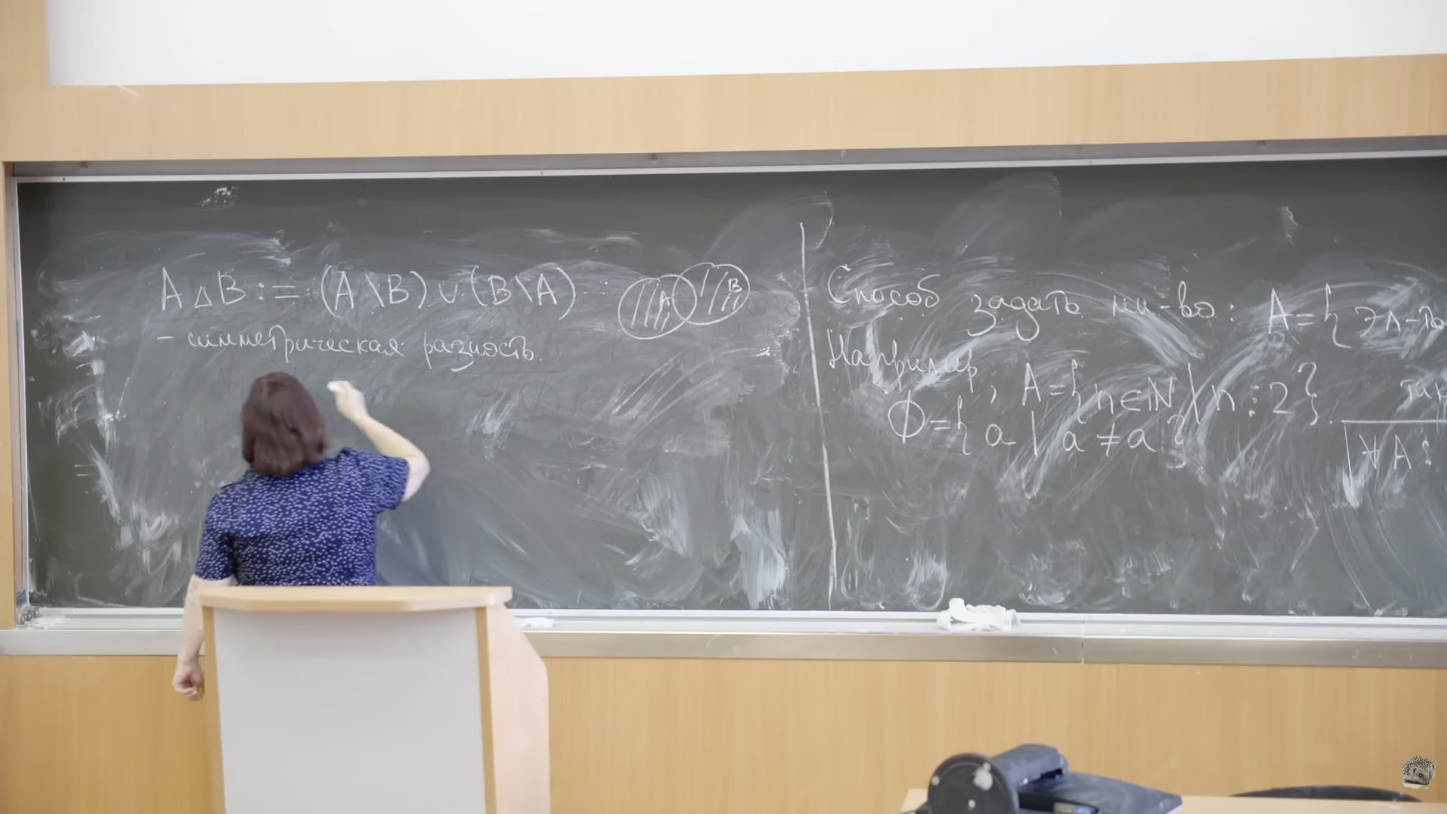
\includegraphics[width=0.47\textwidth]{images/board_chalkboard.png} &
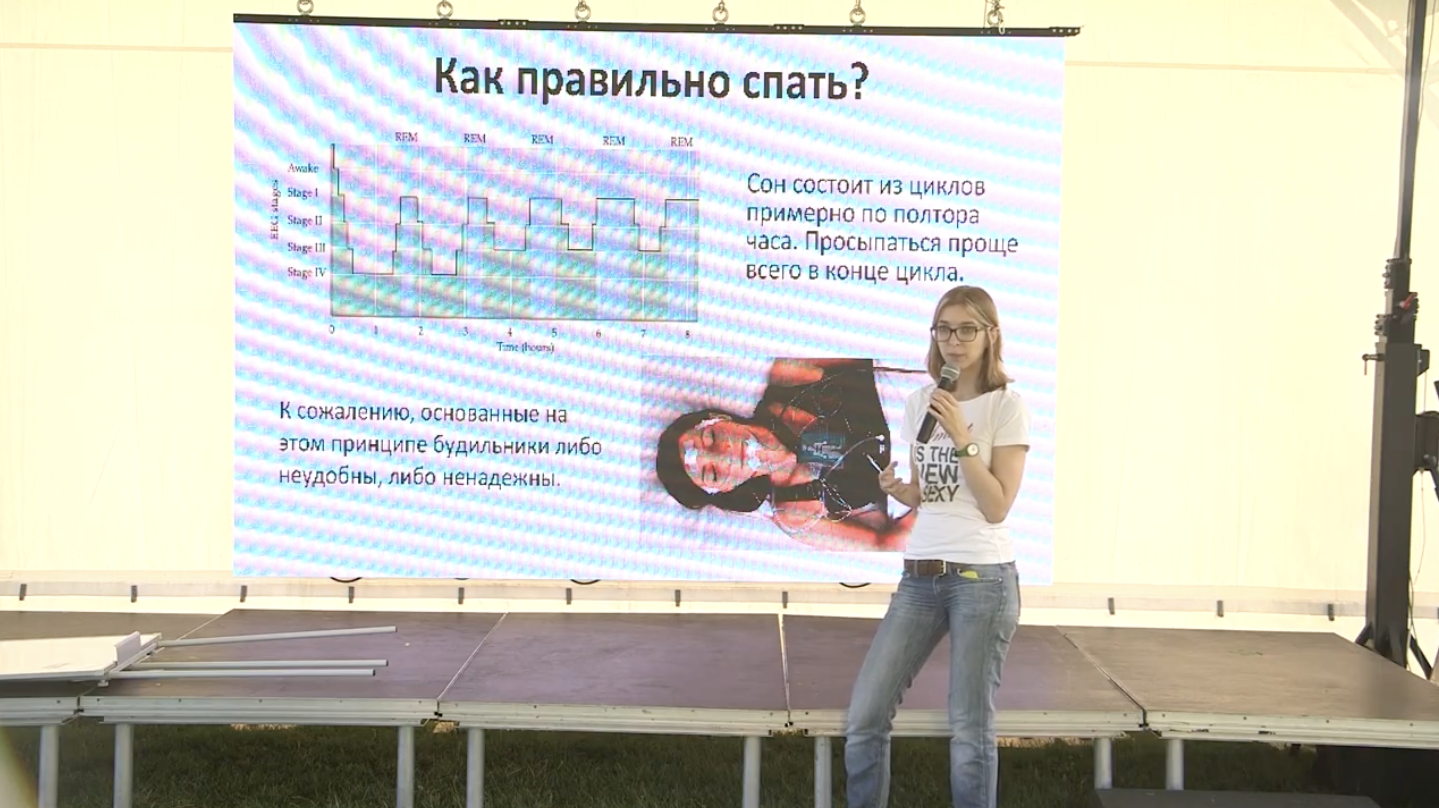
\includegraphics[width=0.47\textwidth]{images/board_screen.png} \\
(a) Меловая доска & (b) Проекционный экран
\end{tabular}

\vspace{4pt}

\small
\begin{tabular}{p{0.20\textwidth} p{0.34\textwidth} p{0.34\textwidth}}
\toprule
 & \textbf{(a) Меловая доска} & \textbf{(b) Проекционный экран} \\
\midrule
\texttt{surface\_type} & blackboard & screen \\
\texttt{readability\_level} & 3 & 3 \\
\texttt{main\_issues} & partial\_obscuration, faint\_writing, smudges & glare, smudges, overexposure \\
Интерпретация & Доска плохо стёрта, часть записей плохо различима. & Артефакты от экрана проектора и камеры, при этом текст читаем. \\
\bottomrule
\end{tabular}

\caption{Два примера с \texttt{readability\_level}~=~3:
одинаковый скор при разных причинах ухудшения читаемости.
Левый кадр — меловая доска (\emph{МГУ, лекция по мат. анализу}),
правый — проекционный экран (\emph{TED-style лекция на открытой площадке}).}
\label{fig:board_readability}
\end{figure}

\paragraph{Агрегация видео скора.}

База — DOVER-скор через сигмоиду (центр~0.4, параметры подобраны эмпирически).
Четыре метрики применяются как мультипликативные штрафы:
резкость (\textit{blur}), мерцание (\textit{flicker}), стабильность (\textit{stability}) и временная консистентность (\textit{consistency})
(высокое стандартное отклонение резкости по кадрам). Каждая метрика переводится в штрафной коэффициент $k_i\in[0,1]$
и при этом суммарный штраф ограничен: $\textit{mult} = \max(0.60, \prod k_i)$.

Читаемость доски добавляется аддитивно, а не мультипликативно.
Логика: штрафы за резкость, мерцание и стабильность относятся к
техническому качеству съёмки — они ухудщают сигнал.
Доска же является содержательным элементом: её читаемость не связана
с качеством съёмки, но напрямую влияет на образовательную ценность видео.
Аддитивная дельта от~$-1.0$ до~$+1.5$ отражает этот вклад отдельно
от технической составляющей.

Для трёх критических дефектов дополнительно применяются условные потолки:
сильное размытие, сильное мерцание или выраженная нестабильность принципиально ограничивают
воспринимаемое качество, и никакие другие характеристики это не компенсируют.

\begin{equation}
\textit{video\_score} = \max\!\bigl(0.5,\;
    \min(\textit{ceiling},\;
    \textit{base} \times \textit{mult} + \textit{board\_delta})\bigr)
\end{equation}

\begin{table}[h]
\centering
\small
\begin{tabular}{lll}
\toprule
\textbf{Компонент} & \textbf{Что входит} & \textbf{Роль} \\
\midrule
$\textit{base}$ & DOVER через сигмоиду & основа \\
$\textit{mult}$ & $k_{\textit{blur}} \cdot k_{\textit{flicker}} \cdot k_{\textit{stability}} \cdot k_{\textit{consistency}}$ & штраф, $\geq 0.60$ \\
$\textit{board\_delta}$ & читаемость доски (Qwen3-VL, 1–5) & бонус/малус, $[-1.0, +1.5]$ \\
$\textit{ceiling}$ & min по blur, flicker, stability & жёсткий потолок \\
\bottomrule
\end{tabular}
\caption{Компоненты агрегации видео скора}
\end{table}

\subsubsection{Агрегация в метрику технического качества}

Итоговый скор технического качества объединяет аудио и видео оценки
через гармоническое среднее:

\begin{equation}
\textit{technical\_score} =
    \frac{2 \times \textit{audio\_score} \times \textit{video\_score}}
         {\textit{audio\_score} + \textit{video\_score}}
\end{equation}

Гармоническое среднее выбрано намеренно: оно автоматически штрафует
асимметрию между компонентами. Арифметическое среднее видео~8/10
и аудио~2/10 даёт 5.0 — результат, не отражающий реальное качество
просмотра. Гармоническое среднее тех же значений даёт~3.2.
Логика та же что и в F1-мере в задачах \texttt{information retrieval},
где гармоническое среднее \texttt{precision} и \texttt{recall} штрафует модели
с сильным дисбалансом между ними: лекция с великолепным видео
но нечитаемым звуком остаётся плохой лекцией.

В \cref{tab:audio_video_examples} приведены примеры из валидационной выборки,
иллюстрирующие разные сценарии соотношения аудио- и видеооценок.

\begin{table}[h]
\centering
\small
\begin{tabular}{p{0.42\textwidth}ccc}
\toprule
\textbf{Сценарий} & \textbf{Аудио} & \textbf{Видео} & \textbf{Итог} \\
\midrule
Студийная запись урока с высоким качеством видео & 6.8 & 9.1 & 7.8  \\
Хорошая запись вузовской лекции & 7.8 & 7.7 & 7.75 \\
Запись преподавателя онлайн-школы с хорошим аудио & 8.1 & 5.3 & 6.4  \\
Старая запись того же канала со слабым видео & 7.3 & 4.3 & 5.4  \\
Вузовская лекция со слабым аудио при приемлемом видео & 4.0 & 6.7 & 4.9  \\
Старая запись вузовской практики с низким качеством обоих каналов & 0.5 & 0.6 & 0.5  \\
\bottomrule
\end{tabular}
\caption{Примеры агрегации аудио- и видеооценок через гармоническое среднее.
Таблица показывает, что итоговый технический скор снижается при дисбалансе между каналами:
при слабом аудио или видео итог оказывается ближе к худшему компоненту, чем к лучшему.}
\label{tab:audio_video_examples}
\end{table}


\subsection{Флаги восприятия}
\label{sec:method-flags}

В \cref{subsec:psychological-functions-flags}~юнговские психологические функции
были обоснованы как теоретическая рамка для декомпозиции понятия
«управление вниманием»: каждая функция описывает доминирующий режим обработки
информации, нарушение которого создаёт специфический тип когнитивного напряжения.
Здесь эта рамка операционализируется в четыре детектируемых флага (по одному на каждую функцию).
Флаг — это бинарный сигнал с параметром уверенности (confidence, 0.0–1.0),
фиксирующий наличие системной проблемы подачи.
Флаги не взаимоисключающие и несколько из них могут сработать одновременно.

Важно что флаги описывают свойства подачи спикера, а не его типа или тип зрителя.
Каждый флаг детектирует нарушение доминирующего канала конкретной функции —
паттерн в поведении лектора, который создаёт когнитивное напряжение 
для людей с данной ориентацией восприятия.
В пользовательском интерфейсе флаги названы иначе, чем юнговские типы:
пользователь видит содержательное описание проблемы,
а не психологическую категорию, 
чтобы исключить ассоциацию с типированием аудитории и упросить взаимодествие.

Перенос типологии из психологической среды в образовательную нетривиален, так как 
Юнг формализует сами психологические функции, но не
какие именно свойства лекционного видео создают дискомфорт для каждой из них.
Для прояснения этих тонкостей был проведён неформальный опрос
в сообществе людей из образовательной среды,
применяющих психологические теории в собственной педагогической практике.
Формат был намеренно неструктурированным, так как цель состояла в сборе мнений
о том, что реально выбивает разных людей при просмотре лекций,
а не в получении стандартизированных ответов — такие вещи плохо
поддаются формализованным анкетам.
Опрос позволил откалибровать соответствие между паттернами подачи
и тем что действительно создаёт дискомфорт для каждой функции,
и в итоге сформировать набор детектируемых паттернов для каждого флага.

Технически флаги неоднородны: часть паттернов детектируется сигнальными
методами — акустическими метриками, компьютерным зрением, анализом движения.
Часть требует понимания смысла: наличие образности в изложении,
характер промежуточных итогов, соответствие эмоционального тона контексту —
классические NLP-методы здесь недостаточны, что будет показано в следующих разделах.
Для таких задач применяется LLM или VLM в формате структурированных промптов.
Во всех флагах, в качестве LLM, используется DeepSeek~V4~\cite{deepseekai2026deepseekv4} в разных модификациях:
модель выбрана за сильные reasoning-способности, надёжную работу
с русскоязычным текстом и стоимость инференса.

\subsubsection{Флаг «Аудио Дисбаланс» (Логик)}

Логический тип воспринимает информацию преимущественно через аудиальный канал,
то есть когда речь или звук мешает восприятию (фоновые шумы, тембральные особенности, слова-паразиты и просторечия) повышается когнетивная нагрузка.
Флаг детектирует два класса проблем: техническую деградацию звука
и речевые паттерны, создающие когнитивную нагрузку при прослушивании.
Компоненты независимы и объединяются через дизъюнкцию —
флаг срабатывает если сработал хотя бы один.

Стоит сказать, что Логик по своей природе системен и последователен, то есть хаотичное повествование создаёт для него дополнительную нагрузку.
Однако структурность изложения является базовым ожиданием от образовательного контента вне зависимости от типа зрителя,
поэтому она не включена в этот флаг как специфичный сигнал и
косвенно рассматривается в рамках педагогического анализа нарративного модуля~(\cref{sec:method-narrative}).

\paragraph{Аудио-компонент.}

Технические метрики звука уже вычислены модулем аудиокачества~(\cref{sec:method-audio}).
Флаг срабатывает, если \texttt{audio\_score}~$< 5.0$.
Этот порог следует из конструкции самой аудио-метрики: \texttt{audio\_score} нормирован на шкалу 0--10,
где значение 5 соответствует границе между условно приемлемым и проблемным качеством речевого канала.
На валидационной выборке такая граница дополнительно проверялась как разумный порог срабатывания флага.
При срабатывании аудио-компонента \texttt{confidence} фиксируется на уровне~$0.95$:
технические метрики дают детерминированный сигнал.

\paragraph{LLM-компонент: речевые паттерны.}

Второй класс проблем — слова-паразиты и нелитературная речь.
Оба явления не поддаются надёжной детекции словарными методами:
паразиты разнообразны и контекстно-зависимы, нелитературные формы
могут быть намеренной авторской интонацией.
Из-за этого компонент построен как проверка устойчивых речевых
паттернов, а не как поиск любых отклонений в устной речи.
Модель LLM анализирует два критерия: слова-паразиты и нелитературные формы речи, 
различая нормальные особенности живого объяснения и повторяющиеся элементы,
которые начинают мешать восприятию.
Для каждого критерия введена трёхуровневая шкала:
\textit{clean}, \textit{natural}, \textit{excessive};
флаг срабатывает только при \texttt{excessive}.
Для снижения ложных срабатываний в промпте явно указано не учитывать
единичные оговорки, техническую терминологию, разговорный стиль подачи
и артефакты сегментации Whisper на границах фраз.
Ответ возвращается в структурированном JSON с уровнем уверенности
и короткими цитатами из транскрипта для каждого сработавшего критерия —
это делает срабатывание флага проверяемым.

\paragraph{Детекция артикуляционных дефектов: неудавшиеся подходы.}

Отдельно исследовалась возможность детектирования артикуляционных особенностей
речи (картавость, нестандартный тембр), так как они создают дополнительную
когнитивную нагрузку на восприятия для логиков, но не улавливаются транскриптом.

Первая гипотеза состояла в использовании \texttt{avg\_logprob} Whisper как прокси-метрики уверенности распознавания.
Предполагалось, что при нестандартном произношении модель будет менее уверенно декодировать речь, и это отразится в более низком среднем log-probability.
Однако на тестовых примерах эта метрика не показала устойчивой связи с артикуляционными особенностями:
видео без выраженных дефектов речи нередко получали более низкие значения \texttt{avg\_logprob}, чем видео с заметной картавостью.
Вероятная причина состоит в том, что уверенность Whisper сильнее зависит от сложности терминологии, темпа речи, качества записи и локального контекста,
чем от самой артикуляционной особенности.
Кроме того, модель достаточно робастна к вариативности произношения и часто корректно транскрибирует такую речь,
не отражая её нестандартность в значении \texttt{avg\_logprob}.

Вторая гипотеза состояла в использовании акустических признаков, рассчитываемых в Praat~\cite{boersma2001praat}: jitter, shimmer и HNR.
Предполагалось, что артикуляционные особенности речи будут отражаться в нестабильности основного тона, амплитуды и гармонической структуры сигнала.
Однако на тестовой выборке эти признаки также не дали устойчивого разделения.
Так, лектор с выраженной картавостью показал jitter~3.17\%, тогда как лектор без заметных артикуляционных дефектов — 4.26\%.
Это показывает, что в условиях естественной YouTube-записи значение признака определяется не только произносительными особенностями,
но и шумом, микрофоном, реверберацией, темпом речи и ошибками выделения voiced-фрагментов.
Вероятная причина заключается в том, что jitter, shimmer и HNR изначально применяются в более контролируемых условиях анализа голоса,
тогда как лекционное YouTube-аудио содержит непрерывную речь, фоновые шумы, компрессию и переменное расстояние до микрофона.
Поэтому в текущей постановке признаки Praat были признаны недостаточно устойчивыми для детектирования артикуляционных особенностей.

Финальная гипотеза состояла в использовании Qwen~Omni с нативным аудиовходом:
тестировались Qwen2.5-Omni-7B локально и Qwen3.5-Omni-Plus через API.
Предполагалось, что мультимодальная модель сможет напрямую оценить не только содержание речи,
но и особенности её звучания.
Однако в тестовых примерах модели возвращали \texttt{false} даже для видео
с заметными артикуляционными особенностями.
Вероятная причина состоит в том, что аудио-LLM в первую очередь оптимизированы
на распознавание и понимание содержания речи, а не на анализ паралингвистических характеристик:
тембра, артикуляции, дикции и индивидуальных особенностей произношения.

Поэтому детектирование артикуляционных особенностей было исключено из текущей реализации
как отдельная нерешённая подзадача.

\subsubsection{Флаг «Смысловая унылость» (Интуит)}

Интуитивный тип воспринимает информацию через движение смыслов.
Хорошая лекция для него — та, где каждый следующий фрагмент добавляет
новый ракурс, поворот или связь: мысль не топчется на месте, а идёт вперёд.
Образность и аналогии (переносы понятий из одной предметной области
в другую) помогают увидеть предмет объёмно, а не плоско.
Промежуточные итоги должны быть синтезом, а не пересказом сказанного.
Важно слышать самого лектора: его интерпретацию, взгляд, личный заход на тему, 
то, чего нет в учебнике и ради чего вообще стоит слушать лекцию, а не читать.
Когда этого нет, а лектор механически озвучивает слайды или учебник, 
интуиту становится скучно вне зависимости от качества звука и картинки.

\paragraph{Промпт и три оси оценки.}

Флаг анализирует транскрипт по трём осям.

\textit{Semantic\_dynamics} — центральная ось: движется ли мысль вперёд.
Каждый следующий фрагмент должен добавлять новое — обобщение, неожиданный ракурс,
выход на следующий уровень понимания. Absent ставится только при устойчивом
паттерне топтания по всей лекции: лектор переливает воду,
дублирует сказанное другими словами, зачитывает то что и так на экране.

\textit{Imagery} — метафоры, аналогии, переносы понятий из одной области в другую,
образные сравнения. Не считается одно техническое определение или вычисление —
речь о том, помогает ли лектор увидеть предмет с разных сторон.

\textit{Own\_voice} — слышен ли сам лектор: его взгляд, интерпретация,
личный пример, неожиданный заход на тему.
Или содержание можно слово в слово прочитать в любом учебнике.

Каждая ось оценивается по шкале \textit{strong / present / absent};
флаг срабатывает только при \texttt{absent}.
Модель обязана приводить цитаты из транскрипта — без них вердикт сложно провалидировать.
В \cref{tab:intuitive-flag-examples} показано, как три оси оценки работают на примерах лекций с разным стилем подачи.

\begin{table}[h]
\centering
\footnotesize
\begin{tabular}{p{0.30\textwidth} p{0.30\textwidth} p{0.30\textwidth}}
\toprule
\textbf{Флаг сработал} &
\textbf{Флаг не сработал} &
\textbf{Флаг не сработал} \\

\textit{БЖД, онлайн-курс} &
\textit{Матанализ, онлайн-школа (для студентов)} &
\textit{Параметры ЕГЭ, онлайн-школа (для школьников)} \\
\midrule

\begin{minipage}[t]{0.30\textwidth}
\footnotesize
\texttt{s\_dyn}: absent\\[2pt]
\textit{«Первая группа~— процессы преобразования веществ... Вторая группа~— процессы создания вещей... Четвёртая группа~— процессы разложения.»}
\end{minipage}
&
\begin{minipage}[t]{0.30\textwidth}
\footnotesize
\texttt{s\_dyn}: strong\\[2pt]
\textit{«Давайте сначала на пальцах это покажем, а потом аккуратно всё докажем.»}
\end{minipage}
&
\begin{minipage}[t]{0.30\textwidth}
\footnotesize
\texttt{s\_dyn}: strong\\[2pt]
\textit{«Мне нужно разобраться, что с этим уравнением происходит. Начну с самой частой области.»}
\end{minipage}
\\[6pt]
\midrule

\begin{minipage}[t]{0.30\textwidth}
\footnotesize
\texttt{imagery}: absent\\[2pt]
\textit{«Структурными элементами техносферы являются технические изделия и территориально-промышленный комплекс.»}
\end{minipage}
&
\begin{minipage}[t]{0.30\textwidth}
\footnotesize
\texttt{imagery}: present\\[2pt]
\textit{«Два милиционера кого-то куда-то ведут.»}
\end{minipage}
&
\begin{minipage}[t]{0.30\textwidth}
\footnotesize
\texttt{imagery}: present\\[2pt]
\textit{«Прямая вот так вот будет ездить вверх-вниз.»}
\end{minipage}
\\[6pt]
\midrule

\begin{minipage}[t]{0.30\textwidth}
\footnotesize
\texttt{own\_voice}: absent\\[2pt]
\textit{«Продолжаем изучать дисциплину безопасности жизнедеятельности. Продолжаем рассмотрение вопросов первого раздела.»}
\end{minipage}
&
\begin{minipage}[t]{0.30\textwidth}
\footnotesize
\texttt{own\_voice}: strong\\[2pt]
\textit{«Я даже не знаю, коснулась ли эту теорему реформа полиции...»}
\end{minipage}
&
\begin{minipage}[t]{0.30\textwidth}
\footnotesize
\texttt{own\_voice}: strong\\[2pt]
\textit{«Дружище, ты должен помнить: параметр~— это задача сильнейших.»}
\end{minipage}
\\

\bottomrule
\end{tabular}
\caption{Спектр оценок флага «Смысловая унылость» на трёх лекциях разного стиля.
Флаг детектирует отсутствие смысловой динамики и авторского голоса,
а не неформальность подачи: академичная лекция и молодёжный курс для школьников
одинаково проходят проверку при разном регистре речи.
Примеры~— цитаты выбранные моделью как иллюстрации вердикта,
а не триггеры срабатывания.}
\label{tab:intuitive-flag-examples}
\end{table}


\paragraph{Эволюция промпта.}

Первая версия флага содержала шесть бинарных вопросов: наличие hook в первые минуты,
метафоры, переформулировки, синтез vs пересказ, авторская позиция,
механические отговорки. Флаг срабатывал при двух и более проблемах.
Подход оказался хрупким: hook нерелевантен для фрагментов длинных курсов,
\texttt{synthesis\_not\_summary} давал ложные срабатывания на математических лекциях
где пересказ ключевого шага перед следующим — нормальная педагогика.
Переход к трём осям с асимметричной агрегацией устранил эти проблемы:
вместо чеклиста критериев модель оценивает целостные характеристики подачи.

\paragraph{Агрегация.}

Агрегация асимметрична: \texttt{semantic\_dynamics = absent} триггерит флаг
самостоятельно — это центральная потребность интуита.
\texttt{imagery} и \texttt{own\_voice} работают в паре:
если оба absent, то лекция является озвучкой учебника,
что само по себе достаточно для срабатывания флага.

\begin{equation}
\begin{aligned}
\textit{flag} ={}&
(\texttt{semantic\_dynamics} = \text{absent}) {}\lor\\
&{}\lor
(\texttt{imagery} = \text{absent}
\;\land\; \texttt{own\_voice} = \text{absent})
\end{aligned}
\end{equation}

\paragraph{Дублирование слайдов и OCR.}

Дублирование слайдов изначально планировалось детектировать отдельным OCR-компонентом.
Код был даже реализован, однако не интегрирован: ось \texttt{semantic\_dynamics}
уже улавливает это через семантику транскрипта —
на видео где лектор дословно читает слайды LLM стабильно возвращает absent.
Ко всему прочему OCR покрыл бы только напечатанный текст на экране, а
для рукописного контента потребовалась бы VLM, что существенно утяжелило бы модуль.
Поскольку семантический подход справился, OCR-компонент остался нереализованным.


\subsubsection{Флаг «Эмоциональный дисбаланс» (Эмоция)}


Эмоциональный тип воспринимает через атмосферу и отношения — ему важна живость и уместность эмоционального тона. Флаг срабатывает в двух противоположных случаях: лектор читает механически без эмоциональной окраски, либо эмоциональный напор не соответствует контексту.

Эмоциональная окраска речи оценивается через модель audEERING \cite{wagner2022transformerser} — трансформерную SER-архитектуру, специально разработанную для закрытия valence gap:
предыдущие поколения SER-моделей стабильно предсказывали arousal, но систематически ошибались по валентности (позитивность / негативность эмоции).
Модель применяется по скользящим окнам на аудиосегментах — вычисляется распределение эмоциональных состояний и их вариативность во времени. Именно вариативность является ключевым признаком:
флаг детектирует не конкретную эмоцию, а её отсутствие или избыток относительно контекста.
Модель обучена на английских данных, однако просодические паттерны эмоциональной речи переносятся между языками устойчиво, что подтверждается в том числе авторами работы.

\subsubsection{Флаг «Визуальный шум» (Сенсорик)}


Сенсорный тип воспринимает через визуальный канал и реальность происходящего в кадре.
Флаг срабатывает когда визуальный ряд перегружен раздражителями: резкие склейки с большим изменением картинки между ними, хаотичное движение в сцене, перегруженность кадра.

Монтажные склейки детектируются через PySceneDetect \cite{castellano2020pyscenedetect} — лёгкий инструмент без зависимостей от нейросетевых моделей,
работающий напрямую на видеопотоке. Резкость перехода оценивается через OpenCV и MediaPipe:
позиция лица лектора сравнивается между кадрами до и после склейки — резкое смещение спикера в кадре является маркером дезориентирующего монтажа.

Общая визуальная опрятность и перегруженность сцены требует семантического понимания картинки
и не поддаётся надёжной формализации через классические дескрипторы — яркость, контраст и оптический поток не улавливают смысловую перегруженность кадра.
Для этой задачи применяется Qwen3-VL.
Тестирование проводилось локально на Qwen3-VL-8B — модель показала достаточное качество на задаче оценки визуальной опрятности при разумном потреблении памяти.
После получения доступа к API принято решение перейти на Qwen3-VL-Plus: это освобождает локальный compute для других модулей пайплайна
и даёт прирост точности без изменения логики модуля.

\subsection{Профиль подачи}
\label{sec:method-profile}

Профиль подачи описывает глобальную педагогическую ориентацию лекции по двум независимым осям: академичность и инструментальность.
Важно, что это не про поверхностные признаки текста — наличие формул, определений или примеров, а скорее про глобальную цель занятия.
Лекция по линейной алгебре на, условном, экономфаке и на матфаке могут иметь близкий лексический состав, иметь теоремы и аксиомы,
но принципиально разную педагогическую ориентацию — одна объясняет чтобы применять, другая строит строгую теорию.

\textbf{Рассмотренные подходы.} Первым был протестирован zero-shot NLI: академичность и инструментальность формулировались как гипотезы, модель возвращала вероятности entailment.
Результатом является полная сатурация: все видео получили 9.5–10.0 по обеим осям.
NLI-модели обучены на формальном entailment общего характера и не различают педагогические ориентации внутри образовательного дискурса
— они фиксируют формальное наличие признаков («в тексте есть определения» значит true), а не глобальную цель занятия.

Следующая попытка — LLM с непрерывной шкалой 0–1. Та же проблема в другом виде: без якорных точек модель не имеет опоры для дифференциации, оценки кластеризовались в узкой зоне.

\textbf{Выбранный подход.} Дискретная пятибалльная шкала с якорными описаниями для каждого уровня.
Академичность: от 1 («разговорное объяснение на пальцах без формальных определений») до 5 («аксиоматическое построение предмета, доказательства, строгая структура понятий»).
Инструментальность: от 1 («объяснение без применения — обсуждает, мотивирует, но не учит действовать») до 5
(«tutorial: пошаговые процедуры, вычисления, код, результат который можно воспроизвести»).
Внутри каждого уровня модель дополнительно выставляет score 0.0–1.0 как точную позицию это даёт непрерывность при сохранении категориальной структуры.

Оси независимы, так как семинар высокого уровня с теорией и задачами может получить 5 по академичности и 4 по инструментальности одновременно.
Модель предоставляет evidence (конкретные цитаты и наблюдения из транскрипта) для каждой оценки для валидации.
Используется LLM с включённым thinking — reasoning-лог показывает что модель действительно анализирует педагогическую структуру, а не просто сопоставляет паттерны.

\subsection{Нарративная суммаризация}
\label{sec:method-narrative}

Нарративный модуль формирует текстовую часть выдачи это компонент системы, который читается как связный текст,
а не набор метрик, и состоит из трёх компонентов: тематической сегментации с таймкодами, педагогического анализа и собственно нарратива.

\textbf{Тематическая сегментация.} Транскрипт разбивается на смысловые блоки с таймкодами и названиями тем.
Гранулярность адаптируется под цель просмотра: пользователь с целью «составить общее представление» получает укрупненные блоки,
пользователь с целью «последовательно изучить тему» — детальную разбивку с таймкодами каждого подраздела.

\textbf{Педагогический анализ.} LLM оценивает структурные характеристики лекции относительно заявленной темы и пользовательского профиля:
пресреквизиты (что нужно знать чтобы смотреть), пробелы в теме (что заявлено в названии но не раскрыто), плотность материала, соответствие названия содержанию.

\textbf{Нарратив.} Неожиданно наиболее нетривиальный компонент.
Задача формулируется так: текст от лица человека, который посмотрел видео и понял в чём его ценность это именно не пересказ тем,
а объяснение что именно примечательно в этом видео для конкретного пользователя с его профилем.
Пересказ («лектор объясняет пределы функций») не помогает принять решение о просмотре, нарратив
(«для бакалавра первого курса который хочет разобраться с нуля — редкий пример где строгость не жертвуется ради доступности») — помогает.

В ходе разработки было установлено что качество нарратива зависит от модели и режима инференса.
Тестировались несколько конфигураций: модели без thinking давали формальные пересказы структуры вместо оценки ценности,
модели с thinking но без достаточного reasoning-бюджета давали поверхностный анализ.
Итоговая конфигурация использует LLM с включённым thinking и достаточным бюджетом токенов на рассуждение — reasoning-лог показывает,
что модель отмечает редкие педагогические приёмы, конкретные понятия, выделяет что отличает видео от аналогичных.

\subsection{Метрика соответствия запросу}
\label{sec:method-relevance}

Метрика соответствия запросу — интегральная оценка по шкале 0–100, агрегирующая все вычисленные компоненты с учётом пользовательского профиля.
Одно и то же видео получает разный балл для школьника и специалиста, для цели «составить общее представление» и «последовательно изучить тему».
Дополнительно учитываются метаданные: соответствие названия содержанию и наличие у канала связанной серии лекций.

Методология взвешивания компонентов находится в разработке: текущие веса подобраны эмпирически на валидационном датасете и требуют дальнейшей калибровки.

\subsection{Пользовательский интерфейс}


Интерфейс решает две задачи: минимизировать усилия пользователя на входе и сделать выдачу интерпретируемой без дополнительного контекста.

Выбор четырёх входных параметров был нетривиальным упражнением: хотелось покрыть ключевые сценарии использования при минимальном количестве полей.
Итоговый набор — роль, уровень образования, погружённость в тему, цель просмотра — признан минимально достаточным после нескольких итераций.

Поскольку пайплайн рисерческий и занимает несколько минут, пользователю отображаются этапы обработки в реальном времени, включая появление транскрипта по мере его готовности.
Важно для ресурсоёмкого процесса, чтобы  пользователь понимал что происходит.

На экране результатов пользовательские параметры остаются видны постоянно, а всё остальное интерпретируется относительно них.
Метрики интерактивны: при нажатии раскрывается описание и интерпретация применительно к конкретному видео.
Флаги реализованы как бинарные индикаторы — числовые шкалы для них не используются, поскольку создавали бы ложное ощущение точности.
Профиль подачи визуализирован как спидометр со смещением от центра, что передаёт доминирующую ориентацию нагляднее двух отдельных чисел.
Таймкоды в нарративной части кликабельны и переключают встроенный YouTube-плеер на нужный момент.
